\chapter{Physics Background}\label{ch:sm}
The Standard Model of particle physics is a $SU(3)\otimes SU(2)\otimes U(1)$ gauge theory that describes the interactions of fundamental particles. It is generally described in two parts, electroweak theory and quantum chromodynamics, presented in the following section. In later sections, the production of \W and \Z bosons in \pp collisions and the modeling of these processes is described. 


%%%%%%%%%%%%%%%%%%%%%%%%%%%%%%%%%%%%%%%%%%%%%%%%%%
%               Standard Model
%%%%%%%%%%%%%%%%%%%%%%%%%%%%%%%%%%%%%%%%%%%%%%%%%%

\section{The Standard Model}\label{ch:sm:sm}
\subsubsection{Introduction}
The SM has been a remarkably successful theory describing fundamental particles and their interactions. The fundamental constituents of matter---leptons and quarks---interact through the strong and electroweak interactions. Depicted in Figure~\ref{fig:intro:sm}, the SM consists of three families of quarks (purple), three families of leptons (green), the force carriers (red), and the Higgs boson (yellow). 

\begin{figure}
\centering
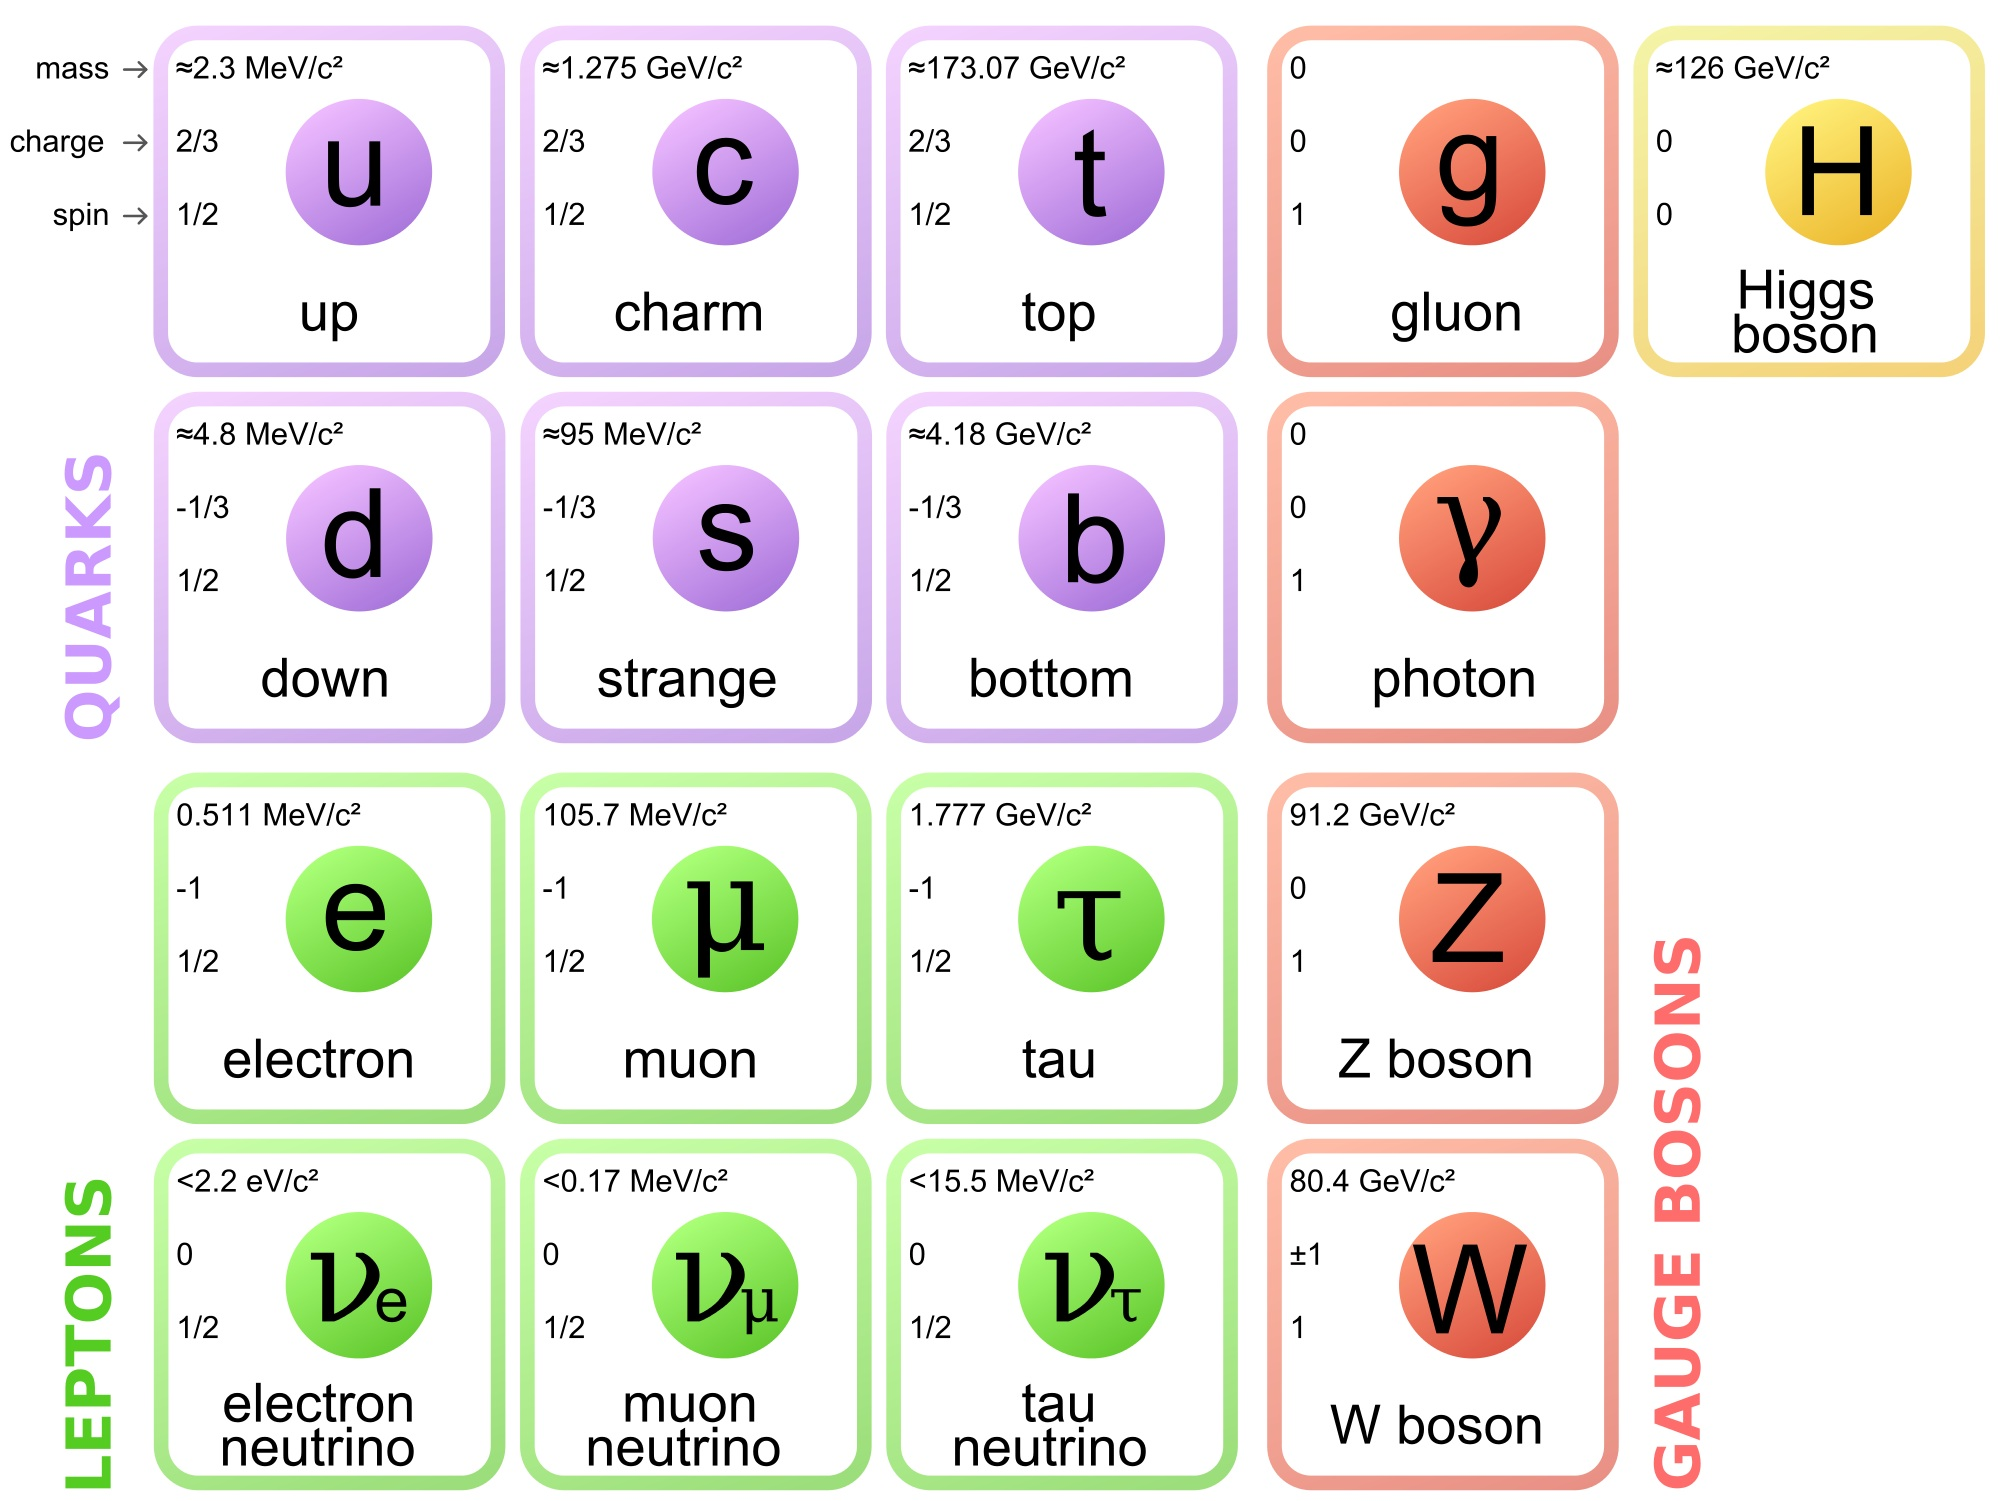
\includegraphics[width=0.6\linewidth]{plots/Intro/sm.jpg}
%   \caption{1a}
%   \label{fig:Eff:el:5TeV:GSFSel:pos
\caption{Fundamental particles of the Standard Model\cite{SM_table}.} \label{fig:intro:sm}
\end{figure}

Familiar building blocks of matter---protons and neutrons---are not the most basic particles, they are composed of constituent quarks and gluons. There are three families of quarks, with six total flavors. Up-type quarks up ($u$), charm ($c$), and top ($t$) have electric charge $+\frac{2}{3} e$, and down-type quarks down ($d$), strange ($s$), and bottom ($b$) have electric charge $-\frac{1}{3}e$. Protons are $uud$, with an electric charge of $+1e$. The strong interaction, mediated by the gluon, binds quarks together into hadrons. The strength of the strong coupling is distance-dependent, with coupling increasing\phil{decreasing or strong coupling at short scales} at long length scales. Therefore, bare quarks have never been observed, as it is favored for them to quickly form bound states. The lepton families are the electron and its more massive analogs, the muon and tau leptons, along with their corresponding neutrinos. 

The weak interaction is propagated by the \W and \Z bosons. Both the charged leptons, neutrinos, and quarks can couple to \W and \Z bosons.  At low energies, the weak interaction is commonly know for its role in beta decay, with uses such as radioluminescent tritium illumination sources and medical imaging positron emission tomography (PET scan).  At energies achieved by the LHC, the \W and \Z bosons can be produced in $pp$ collisions and the properties of the production can be studied. As described in below, this provides important information on several fronts, including event modeling and detector performance.


%%%%%%%%%%%%%%%%%%%%%%%%%%%%%%%%%%%%%%%%%%%%%%%%%%
%                     ewk
%%%%%%%%%%%%%%%%%%%%%%%%%%%%%%%%%%%%%%%%%%%%%%%%%%

\subsection{Electroweak Theory}\label{ch:sm:ewk}
In the SM\cite{SMEWK1,SMEWK2,SMEWK3}, electroweak interactions belong to the gauge group $SU(2) \otimes U(1)$, with the gauge bosons $W_{\mu}^i$ ($i = 1,2,3$) for $SU(2)$ and  $B_{\mu}$ for $U(1)$.  The left-handed fermions transform as doublets, where the leptons are given in Equation~\ref{eq:phys:ewk:leptons} and quarks are shown in Equation~\ref{eq:phys:ewk:quarks}. The $d_i'$ are given by $d_i' = \sum_j V_{ij} d_i$, where $V_{ij}$ are the elements of the Cabibbo-Kobayashi-Maskawa (CKM) matrix\cite{ckm1,ckm2}.
\begin{equation}
  \Psi=\binom{v_e}{l_e},~\binom{v_{\mu}}{l_{\mu}},~\binom{v_{\tau}}{l_{\tau}}
  \label{eq:phys:ewk:leptons}
\end{equation}
\begin{equation}
  \Psi=\binom{u}{d'},~\binom{c}{s'},~\binom{t}{b'}
  \label{eq:phys:ewk:quarks}
\end{equation}
Vector fields corresponding to particles with spin 1 and mass are the $W_\mu^\pm$, $Z_\mu$, and photon $A_\mu$, which are given in terms of the gauge fields as:
\begin{equation}
\begin{aligned}
    &A_\mu = B\mu cos\theta + W^3_\mu sin\theta\\
&Z_\mu = -B\mu sin\theta + W^3_\mu sin\theta\\
&W_\mu^\pm = W_\mu^1 \mp i W^2_\mu
\end{aligned}
\label{eq:ewk_s1_particles}
\end{equation}

Mass generation is achieved through spontaneous symmetry breaking of $SU(2)\otimes U(1)$ to $U(1)_{em}$ with the addition of a complex scalar doublet $\phi = \frac{1}{\sqrt{2}}\binom{\sqrt{2}\phi^+}{\phi^0 + ia^0}$, known as the Brout-Englert-Higgs mechanism\cite{ewsb1,ewsb2,ewsb3}. The potential is given by $V(\phi) = \mu^2\phi^\dagger\phi + \lambda^2(\phi^\dagger \phi)^2$, with the full Lagrangian being given in Equation~\ref{eq:lagrangian_higgs}. With $\mu^2 < 0$, the vacuum expectation value of $\phi$ is $<\phi> = v/\sqrt{2} = \mu/\lambda$ with $v\approx 246$ GeV. 
\phil{I would call below $\mathcal{L_{Higgs}}$}

\begin{equation}
    \mathcal{L} = (D_\mu\Phi)^\dagger(D^\mu\Phi) - \mu^2 \Phi^\dagger\Phi - \lambda(\Phi^\dagger\Phi)^2
    \label{eq:lagrangian_higgs}
\end{equation}
The covariant derivatives of Equation~\ref{eq:lagrangian_higgs}, $D_\mu\Phi$, provide the couplings between the Higgs fields and the $W_\mu$ and $B_\mu$ gauge fields, shown in Equation~\ref{eq:covariant_deriv}
\begin{equation}
    D_\mu \Phi = (\partial_\mu + ig\sigma^aW_\mu^a/2 + ig'YB_\mu/2)\Phi
    \label{eq:covariant_deriv}
\end{equation}
Three of the four degrees of freedom introduced by the Higgs doublet are absorbed into the $W^i_\mu$ and $B_\mu$ fields of the $SU(2)\otimes U(1)$ and become the longitudinal components of the \W and \Z bosons. The physical \W and \Z bosons also acquire mass. The generator of the unbroken $U(1)_{em}$ gauge symmetry, the photon, remains massless. The remaining degree of freedom manifests as the new neutral scalar particle, the Higgs boson. The masses of the physical bosons are given in Equation~\ref{eq:boson_masses}.
\begin{equation}
\begin{aligned}
m_H &= \lambda v \\ 
m_W &= \frac{1}{2}g v = cos\theta_W m_Z \\ 
m_z &= \frac{1}{2}\sqrt{g^2+g'^2}v  = \frac{M_W}{\cos{\theta_W}}\\ 
m_\gamma &= 0
\end{aligned}
\label{eq:boson_masses}
\end{equation}
Fermion masses are likewise given through a Yukawa coupling to the Higgs field, shown in Equation~\ref{eq:yukawa}. Fermion masses become $m_{f_i} = h_{f_i} v / \sqrt{2}$ after rotation into a basis where the Higgs-fermion interaction is diagonalized. The fermion coupling to the Higgs boson is $\frac{m_f}{v}\bar{f}fH$, proportional to its mass.
\begin{equation}
\mathcal{L}_{yukawa} = -\hat{h}_{d_{i,j}}\bar{q}_{L_i}\Phi d_{R_j} - \hat{h}_{u_{i,j}}\bar{q}_{L_i}\bar{\Phi} u_{R_j} -\hat{h}_{l_{i,j}}\bar{l}_{L_i}\Phi e_{R_j} + h.c.
    \label{eq:yukawa}
\end{equation}
In Equation~\ref{eq:yukawa}, $q_L$ and $u_R,d_R$ are the quark doubles and singlets, and $l_L$ and $e_R$ are the lepton doublets and singlets. As the Higgs boson is electromagnetically neutral and also transforms as a singlet in $SU(3)$, there are no tree-level couplings of the Higgs to either photons or gluons.

%%%%%%%%%%%%%%%%%%%%%%%%%%%%%%%%%%%%%%%%%%%%%%%%%%
%                     qcd
%%%%%%%%%%%%%%%%%%%%%%%%%%%%%%%%%%%%%%%%%%%%%%%%%%

\subsection{Quantum Chromodynamics}\label{ch:sm:qcd}

The strong interaction between quarks and gluons is described by quantum chromodynamics (QCD), the $SU(3)$ part of the SM. Interactions between quarks and gluons is described by the Dirac Lagrangian density given in Equation~\ref{eq:qcd_lagrangian}. Quarks and gluons carry color charges (red, green, or blue: $N_C = 3$), and there are eight color-combinations of gluons as mediators of the strong force ($A^C_\mu$,~$C=[1...8]$). Quarks are represented by the $\bar{\psi}_{f,\alpha}$ spinors, with the six flavors of quarks ($u,c,t,d,s,b$) represented by $f$, the three colors by $\alpha$, and the quark masses by $m_f$.
\phil{You forgot $\psi$ ie $\gamma_{f,\beta}\psi_{f,\alpha}$}

%% QCD Lagrangian
\begin{equation}
    \mathcal{L}=\bar{\psi}_{f,\alpha}(i\gamma^\mu \partial_\mu \delta_{\alpha\beta}-g_s\gamma^\mu t^C_{\alpha\beta}\mathcal{A}^C_\mu-m_f\delta_{\alpha\beta})\gamma_{f,\beta}-\frac{1}{4}F^b_{\mu\nu}F^{b,\mu\nu}
    \label{eq:qcd_lagrangian}
\end{equation}
%% %% Full Lagrangian
% \begin{equation}
%     \mathcal{L}=\bar{\psi}_{f,\alpha}(i\gamma^\mu \partial_\mu \delta_{\alpha\beta}-g_s\gamma^\mu t^C_{\alpha\beta}\mathcal{A}^C_\mu-m_f\delta_{\alpha\beta})\gamma_{f,\beta}-\frac{1}{4}F^b_{\mu\nu}F^{b,\mu\nu}-\theta\frac{g^2_{s}}{72\pi^2}\epsilon_{\mu\nu\rho\sigma}F^{c,\mu\nu}F^{c,\rho\sigma}
%     \label{eq:qcd_lagrangian}
% \end{equation}
 The eight generators of the $SU(3)$ color group are $3\times 3$ matrices $t^C_{\alpha\beta}$. The strong coupling constant is $g_s$ ($\sqrt{4\pi\alpha_s}$), where $\alpha_s$ varies with energy scale.  The gluon field tensors $F_{\mu\nu}$ are shown in Equation~\ref{eq:qcd_field_tensors}, where the $f_{ABC}$ are the structure constants of $SU(3)$.
\begin{equation}
F_{\mu\nu}^A = \delta_{\mu} \mathcal{A}^A_{\nu} - \delta_{\nu} \mathcal{A}^A_\mu - g_s f_{ABC} \mathcal{A}_\mu^B \mathcal{A}_\nu^C,~~~~ [t^A, t^B] = if_{ABC}t^C
\label{eq:qcd_field_tensors}
\end{equation}
The parameters of QCD are the quark masses ($m_f$) and the coupling constant ($g_s$). There is an additional term in the QCD Lagrangian which is not included in Equation~\ref{eq:qcd_lagrangian}, which contains a parameter $\theta$, and allows for CP violation in QCD. Experimental limits on the neutron electric dipole moment constrain this term to be $\theta < 10^{-10}$ \cite{PhysRevLett.97.131801}.

Computational methods for QCD predictions include lattice gauge theory and perturbative expansion methods. Feynman rules for QCD allow diagrams with $q\bar{q}g$ and $ggg$ vertices and a $gggg$ vertex\cite{Ellis:1991qj}. Perturbative QCD (pQCD) expresses predictions for observables as an expansion in terms of the coupling $\alpha_s(\mu_R^2)$ i.e. $f = f_0 + f_1\alpha_s + f_2\alpha_s^2 + f_3\alpha_s^3 +....$. The coupling $\alpha_s(\mu_R^2)$ is a function of the renormalization scale $\mu_R$, and the effective strength of the interaction with momentum transfer $Q^2$ is $\alpha_s(\mu_R^2 \sim Q^2)$. Calculations are done with Feynman diagrams and are generally performed to only a few terms---leading order (LO, first term), next-to-leading order (NLO, first two terms), and so forth.
The scale dependence of QCD is expressed in the renormalization group equation:
\begin{equation}
    \mu^2_R\frac{d\alpha_s}{d\mu_R^2} = \beta(\alpha_s) = -(b_0 \alpha_s^2 + b_1 \alpha_s^3 + b_2 \alpha_s^4 + \cdots)
    \label{eq:renormalization_group}
\end{equation}
%where $b_0$ is the 1-loop coefficient, $b_1$ is the 2-loop coefficient, etc. 
The minus sign indicates that the coupling becomes weak for interactions with high momentum transfer and is strongly interacting for low energy scales, the source of asymptotic freedom \cite{PhysRevLett.30.1346, PhysRevLett.30.1343}. Values of $\alpha_s$ range from $\alpha_s \sim 0.1$ for $Q$ in the $100 \GeV - \TeV$ range to over $\alpha_s \sim 0.3$ for processes with momentum transfer $Q \sim 1 \GeV$, as depicted in Figure~\ref{fig:sm:alpha_s}. Free quarks have not been observed---they quickly hadronize into mesons or baryons on the time scale $\sim 1/\Lambda$, while the top quark decays before hadronization. This is understood as a result of the strong coupling increasing at low energies (large distance scales), and only the color-singlet hadrons are observed.
\begin{figure}[htbp]
\centering
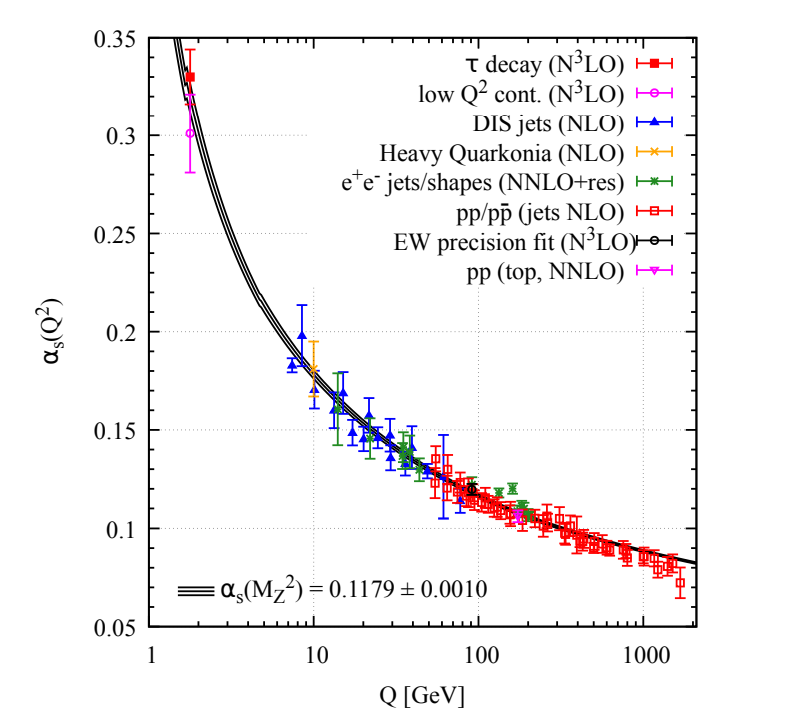
\includegraphics[width=0.6\linewidth]{plots/SM/a_s.png}
\caption{Measurements of $\alpha_s$ demonstrating the scale-dependence\cite{PhysRevD.98.030001}.}
\label{fig:sm:alpha_s}
\end{figure}